
{

\Hide
\chapter{Antecedentes Generales}
}

\begin{titular} 
	\uppercase{
	capítulo 2 \\
	Antecedentes Generales \\
	}
\end{titular}


\section{Votación electrónica}
\subsection{Definición}

En la literatura existen diversas definiciones sobre la votación electrónica, algunas de éstas son
muy amplias, en este trabajo se refiere a ``donde el registro, interpretación o conteo de los votos
en elecciones y referendums políticos involucra tecnologías de información y comunicación'' 
\cite{InternationalInstituteforDemocracyandElectoralAssistance2011}. 


Existe un modelo general del proceso eleccionario el cual descansa en el Pacto Internacional de Derechos Civiles y Políticos
adoptado por las Naciones Unidas el 16 de diciembre de 1966, el cual en su artículo 25 define 8 
principios para las elecciones las cuales describen todo el proceso electoral y que \cite{Hinz2003} los organiza 
en 3 períodos: 

\begin{figure}[h!]
	\centering
	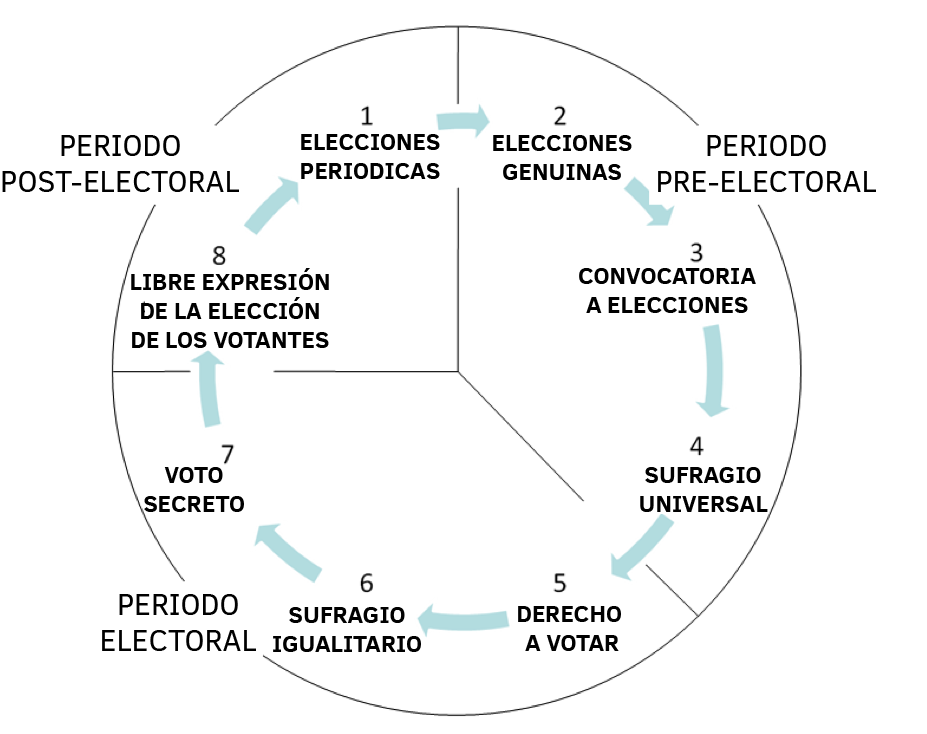
\includegraphics[width=0.7\textwidth]{figura-ciclo}
	\caption[Ciclo del proceso electoral]{Ciclo del proceso electoral. Adaptado de \protect\cite{Hinz2003}}
	\label{fig:tipos-votacion}
\end{figure}
\bigskip

El \textit{período pre-electoral} es el período desde la llamada a elecciones hasta el comienzo de la votación, 
el \textit{período electoral} es el día, o los días, donde los votantes ejercen su derecho a voto y el 
\textit{período post-electoral} es el período donde los resultados son anunciados y una nueva elección es llamada.

Los procesos eleccionarios, ademas de diferenciarse según regulaciones legales de cada país, 
se diferencian según la forma de cómo lo llevan a cabo. En la figura~\ref{fig:tipos-votacion} podemos ubicar la 
votación electrónica y sus dos variantes: en estación y por internet, también llamada remota.

\begin{figure}[h!]
	\centering
	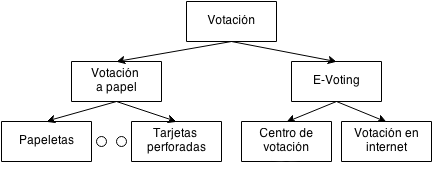
\includegraphics[width=0.7\textwidth]{figura-clasificacion}
	\caption[Clasificación de tipos de votación]{Clasificación de tipos de votación, adaptado de \cite{Kosmopoulos2004}}
	\label{fig:tipos-votacion}
\end{figure}
\bigskip

Las votaciones electrónicas se pueden clasificar dependiendo del tipo de tecnología 
que se utiliza, \cite{InternationalInstituteforDemocracyandElectoralAssistance2011} 
identifica 4 tipos de sistemas de votación electrónica

\begin{itemize}
	\item \textbf{Máquinas DRE}: En inglés ``Direct recording electronic voting machines''. Son máquinas que 
	registran el voto directamente en el sistema. Pueden usarse con o sin documentos (paper trail),
	 los cuales son usados para proveer evidencia física del voto.
	
	\item \textbf{Sistemas OMR:} OMR es un acrónimo de ``Optical Mark Recognition''. Estos sistemas están basados en 
	máquinas que reconocen la opción del votante mediante el escaneo de papeletas con formato especial. (En Chile se usan
	para la PSU )
	
	\item \textbf{Impresoras de papeletas electrónicas:} Similares a las máquinas DRE, estas máquinas producen un papel o ítem
	electrónico con la opción del votante, las cuales son ingresadas a un escáner que contabiliza el voto.
	º
	\item \textbf{Sistemas de voto por internet:} Los votos son transferidos via internet a un servidor central. Los votos pueden 
	ser enviados desde una estación pública o desde cualquier computador conectado a internet.
	
\end{itemize}



%El funcionamiento de la votación por estaciones es similar a la 
%v%otación tradicional, donde el votante se desplaza a lugares autorizados
%a votar, mientras que la votación remota se refiere a poder votar
%desde dispositivos conectados a internet. Una de las ventajas de
%la votación remota en comparación de la votación es en estación es
%que las personas que están imposibilitados de desplazarse puedan
%sufragar.


%La votación remota tiene sus propios problemas, una de sus mayores
%amenazas de seguridad es la posibilidad de que exista \textit{malware} en
%la máquina donde el votante sufraga. Malware puede ser fácilmente diseñada
%para prevenir que el usuario vote, para violar la privacidad enviando
%la elección del usuario a un tercero o para alterar el voto de tal forma que 
%no sea contado en la elección. \cite{Yasinsac2013}.

\newpage
\subsection{Conceptos}

Para entender los trabajos en el tema, es necesario entender algunos
conceptos. Usualmente los estudios suelen definir su propio conjunto de términos
que son utilizados en las investigaciones respectivas, pero existe cierto consenso
en algunos conceptos básicos. En este trabajo se utilizan ciertos conceptos que 
\cite{Yumeng2012,Goodman2012} los define en la siguiente lista:

\begin{itemize}
	\item \textbf{Votante:} Una persona que es elegible para votar
	
	\item \textbf{Candidato:} Una persona que es elegido para ser votado para una posición.
	
	\item \textbf{Papeleta y recibo:} La papeleta está diseñada para una elección 
	específica y es usada para elegir el candidato. Votantes pueden 
	usar el recibo para verificar que su voto ha sido recolectado correctamente.
	
	\item \textbf{Autoridad de registro:} La oficina que examina si un votante es elegible.
	
	\item \textbf{Autoridad de conteo:} La oficina que recibe y verifica los 
	votos, para luego calcular y producir los resultados de la votación
	
	\item \textbf{Escrutador:} La persona que gestiona y supervisa el proceso de votación
	
	\item \textbf{Tabla de anuncios y canal de comunicación:} La tabla 
	de anuncios es usada para publicar información relacionada, como el 
	padrón electoral, votos cifrados y resultados. El canal de comunicación, 
	que puede ser anónimo, es usado en sistemas de votación remota.
	
	\item \textbf{Máquina DRE:} Una máquina de registro electrónico directo de votos (Direct Recording Electronic Voting Machine)
		registra directamente la elección del votante en cada balotaje. Lo hace a través de una papeleta
		que aparece en una pantalla. Generalmente estas máquinas tienen pantallas planas táctiles o 
		con un teclado. Lo que define a estas máquinas es que los votos son capturados y almacenados
		electrónicamente.
		
\end{itemize}
		
\newpage
\subsection{Requisitos de la votación electrónica}

Como vimos anteriormente, las Naciones Unidas tiene definido un conjunto de principios
relativos a los procesos eleccionarios los cuales los miembros firmantes deben cumplir.
En Europa han avanzado aún más en la definición de derechos y deberes de los estados
miembros con respecto a las elecciones. El artículo 3 del protocolo 1 de la convención europea sobre 
derechos humanos \cite{EuropeanCourtofHumanRights2013} dice: 
``Las Altas Partes contratantes se comprometen a celebrar elecciones libres a 
intervalos razonables usando voto secreto, bajo condiciones que aseguren la libre
expresión de las personas en la elección del cuerpo legislativo''. 

Además, la comisión de Venecia del consejo de Europa  \cite{CouncilofEurope-VeniceCommission2002}
 produjo un código de buenas prácticas en materias electorales: En el artículo 4 acerca del sufragio 
secreto, dice que ``el secreto del voto no es sólo un derecho sino también un deber, el 
incumplimiento de este debe ser sancionado con la inhabilitación 
de papeletas cuyo contenido se diera a conoce''. También es dicho que ``La votación debe
ser individual. La votación familiar y cualquier otra forma de control de un votante
sobre otro debe ser prohibido''.

Estas obligaciones en su conjunto conforman una serie de requisitos que la
votación electrónica debe satisfacerlos. Es por esto que es crítico garantizar el correcto funcionamiento 
de los sistemas de votación electrónica, abordando las amenazas como compra de votos y 
estableciendo mecanismos que permitan verificar la integridad del resultado de la elección \cite{Weber} . 
Dadas estas razones es que varios autores proponen una serie de requisitos que deben ser 
satisfechos al implementar sistemas de votación electrónica. Estos ``requisitos'' no se deben confundir
con requerimientos de software, puesto que los primeros no necesariamente involucran software.

Usualmente cada propuesta de sistemas de votación electrónica define su propio conjunto
de requisitos a satisfacer, \cite{Cetinkaya2008} explica que varios estudios han definido informalmente 
una lista de requerimientos para la votación electrónica y propone formalmente
8 requisitos fundamentales a considerar para protocolos de votación 
electrónica: \textit{privacy, eligibility, uniqueness, fairness, uncoercibility,
receipt-freeness, accuracy e individual verifiability}. Pese a esto,
existen ligeras diferencias al definir los requisitos entre distintos estudios, y varias de
estas definiciones son incompatibles con otros modelos de votación electrónica \cite{Braunlich2013}. 

En la siguiente lista se definen los requisitos que más se repiten en la literatura de acuerdo 
a lo mostrado por \cite{Foster2004,Yumeng2012}:

\begin{itemize}

	\item \textbf {Completeness:} Todos los votos válidamente
	emitidos son recolectados correctamente.

	\item \textbf {Soundness:} Prevenir que usuarios maliciosos alteren 
	el sistema de forma tal que no pueda funcionar de la forma correcta.

	\item \textbf {Privacy:} Los votos no pueden ser relacionados a la 
	persona que la emitió.

	\item \textbf {Unreusability:} Un votante sólo puede emitir un sólo voto válido.

	\item \textbf {Eligibility:} Ninguno de los votantes habilitados puede ser impedido de votar

	\item \textbf {Convenience and efficiency:} La votación debería ser “fácil” para 
	votantes sin conocimiento de encriptacion y otras tecnologías.
	
	\item \textbf {Receipt-freeness:} La imposibilidad de probar que un votante votó 
	de cierta manera, aún cuando el votante quiera.

	\item \textbf {Coercion-resistance:} Implica receipt-freeness, ademas de 
	considerar ataques del mundo real relacionados con la coerción, como la 
	compra de votos.

	\item \textbf {Fairness:} Los resultados intermedios de la 
	eleccion no deben ser revelados, evitando que se muestren 
	candidatos como ganadores antes de serlo.

	\item \textbf {Verifiability:} Verificación universal se 
	refiere a que todos pueden verificar la elección. Verificación local se 
	refiere a que sólo el votante puede verificar su voto en la elección.  

\end{itemize}

La idea de definir estos requisitos es establecer un marco de trabajo por el 
cual las implementaciones se rigen. Actualmente no existen estándares
y requisitos globalmente aceptados, entonces cada país debe
definirlos basado en los acuerdos legales alcanzados internacionalmente, 
los cuales fueron expuestos anteriormente, para poder ser implementados y adoptados
en procesos eleccionarios \cite{InternationalInstituteforDemocracyandElectoralAssistance2011}. 

No todos los requisitos anteriormente expuestos pueden ser satisfechos al mismo tiempo, y como 
indica \cite{Langer2010}, las propuestas suelen enfocarse en satisfacer un subconjunto 
de todos los requerimientos expuestos y balancean el cumplimiento para lograr
sistemas que se puedan poner en práctica.


\newpage
\section{Sistemas de votación electrónica}

\subsection{Descripción}

Como vimos anteriormente, si bien existe un marco legal aceptado internacionalmente
sobre el proceso eleccionario, existen diferencias al traducirlo a un conjunto de requisitos que los sistemas de votación
electrónica deben satisfacer. A partir de un modelo general del proceso eleccionario 
que sirve para abstraerse de todas estas diferencias, \cite{Ikonomopoulos2002} define un 
diagrama de casos de uso de un sistema de votación electrónica genérico:

\begin{figure}[h!]
	\centering
	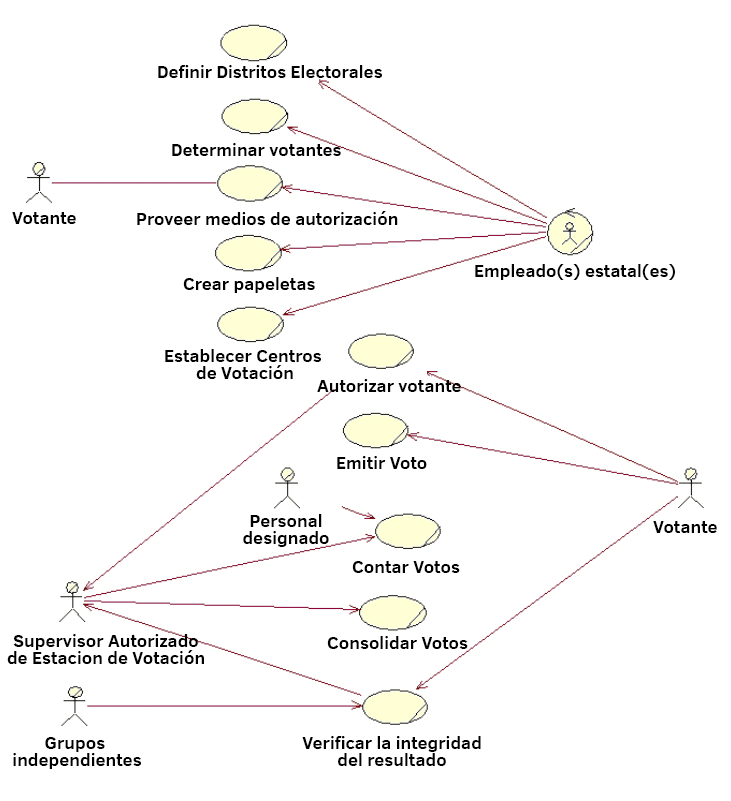
\includegraphics[width=0.7\textwidth]{figura-usecases2}
	\caption[Casos de uso para un modelo general de elecciones generales]{Casos de uso para un modelo general de elecciones generales, adaptado de \cite{Ikonomopoulos2002}}
	\label{fig:casos-uso}
\end{figure}

\begin{itemize}

	\item \textbf{Definir distritos electorales:} Este proceso es ejecutado
		al principio de la elección para definir los distritos y su
		correspondiente número de candidatos que postulan a ser
		representantes. Un distrito electoral es una región del país que
		elige a sus propios representantes.
		
	\item \textbf{Determinar votantes:} En este proceso se lista a todas
		las personas elegibles de ir a votar. Generalmente depende 
		de la regulación legal de la elección.
	
	\item \textbf{Proveer medios de autentificación:} En este proceso
		se provee a los electores de una forma de poder identificarse
		a si mismos durante la elección. En algunos países esto no
		ocurre puesto que se usa la tarjeta de identificación (carnet) o
		el pasaporte. 
	
	\item \textbf{Establecer centros de votación:} Este proceso busca 
		proveer la infraestructura necesaria, tanto en personas como
		en equipamiento, para permitir la ejecución de la elección.
	
	\item \textbf{Crear papeletas:} En este proceso se genera una lista
		con los representantes a elegir según distrito electoral, para 
		luego distribuirla a los centros de votación pertinentes.
	
	\item \textbf{Autorizar votante:} Este proceso se ejecuta cuando un 
		votante procede a un centro de votación. A fin de que el votante
		es elegible y que es el mismo quien votará, se autentifica usando
		el medio de autentificación determinado.
		
	\item \textbf{Emitir votos:} En este proceso la persona vota en una 
		forma que proteja su privacidad y que se registre su voto.
		
	\item \textbf{Contar votos:} En este proceso se busca validar los votos
		emitidos y contar cuantos votos ha recibido cada representante,
		incluyendo los inválidos.
		
	\item \textbf{Consolidar votos:} Este proceso busca concentrar los
		votos contados junto con la lista de las personas que votaron
		desde los centros de votación hacia un repositorio central.
	
	\item \textbf{Verificar la integridad del resultado:} Este proceso ocurre
		cuando un votante o cualquier grupo pide verificar que todos los
		procesos de la elección han sido conducidos adecuadamente.

\end{itemize}

Otro enfoque que nos permite comprender los sistemas de votación electrónica es el 
enfoque ortogonal. De esta manera se pueden dividir los sistemas de votación electrónica en
4 capas, las cuales están constituidas por \textit{componentes}. 
La conveniencia de esta clasificación es que cada componente
puede tener su propio análisis de amenazas y estrategia de verificación,
disminuyendo los riesgos del sistema completo al hacer cambios a
sólo a alguna parte \cite{Lundin2010}.

\begin{table}[h!]
\centering
\begin{tabularx}{\textwidth}{p{3.5cm} X} 
\toprule[1.5pt]
	\bf 	Capa	& \bf 	Componentes 	\\ \hline
	\multirow{4}{*}{Capa humana}        		&	Registro de votantes	\\
									&	Configuración de formulario de papeleta	\\
									&	Administración de estación de votación \\
									&	Verificación de “front-end” \\ \hline 
	\multirow{3}{*}{Capa de elección}		&	Método de elección	\\
									&	Sistema de administración de elección	\\
									&	Canal de comunicación de caja de papeletas \\  \hline
	\multirow{3}{*}{Capa computacional}	&	Esquema de cifrado	\\
									&	Estrategia de anonimato \\
									&	Procedimiento de conteo \\  \hline				
	\multirow{3}{*}{Capa física}			&	Método de autenticación por hardware \\
									&	Estrategia de publicación \\
									&	Método de transferencia \\ 
					
\bottomrule[1.25pt]
\end{tabularx}
\caption[Tabla de componentes de sistemas de votación electrónica]{Tabla de componentes de sistemas de votación electrónica, adaptado de \cite{Lundin2010}}
\label{tab:componentes}
\end{table}


La siguiente es una lista con las 4 capas de un sistema de votación 
electrónica y su descripción. La lista de componentes por capa están definidos 
en la tabla~\ref{tab:componentes}:

\begin{itemize}
	\item \textbf {Capa humana} En esta capa están presentes los aspectos
		del sistema que están en contacto con el votante, como el registro
		de votantes y las estaciones de voto y su manejo.	
	
	\item \textbf {Capa de elección:}  Esta capa es derivada de las leyes que 
		gobiernan la elección, puesto que están presentes componentes
		que pueden no transformarse en software, o que corresponden a 
		software externos. Principalmente están presentes la administración
		de la elección y las definiciones de alto nivel del sistema de votación,
		de forma que tanto los desarrolladores como el publico general entienda
		la dinámica de la elección.
			
	\item \textbf{Capa computacional:} En esta capa se incluyen todos los procesos
		realizados implícitamente por software, incluyendo principalmente los 
		métodos criptográficos y los procedimientos de conteo.
			
	\item \textbf{Capa física:} Es la capa más básica y soporta las demás capas
		con la infraestructura física para facilitar el hardware ocupado en los distintos
		aspectos del sistema.	
\end{itemize}


La definición de estas 4 capas, más los casos de uso anteriormente presentados, nos dan un
cuadro general de los sistemas de votación electrónica que más adelante serán asociados
con requerimientos no funcionales de acuerdo a un modelo de calidad de software, ya que por ejemplo la capa humana
guarda directa relación con la característica de Operability, ya que ambas se refieren a
la interacción entre los recursos humanos y el sistema electrónico. 

% estilos para el documento %
\setlength{\parindent}{1cm}
\setlength{\parskip}{5pt}

\newpage
\subsection{Adopción y situación actual}

En la actualidad, existe la creencia generalizada que cualquier organización que no incluya
tecnología en sus procesos estará pronto obsoleta. Pese a que las naciones tratan sus elecciones
como un proceso delicado y frágil, el que hay que cuidar, el tema de como adaptar la tecnología
existente para mejorar las elecciones de gobernantes es inevitable. Los beneficios que significaría 
reemplazar los procedimientos de voto con dispositivos electrónicos es que se reducirán los 
costos de las elecciones, se acelerará el conteo de votos y facilitará la participación en la elección, 
además de un aumento en la participación dará a lugar a que las elecciones tengan 
resultados más confiables \cite{Kucharczyk2010}.

Para que la votación electrónica sea adoptada, según \cite{InternationalInstituteforDemocracyandElectoralAssistance2011} 
es necesario que el público confíe en el sistema. Lograr que el público confíe en las elecciones
depende de muchos factores, la figura~\ref{fig:piramide} nos ayuda a comprender los distintos 
factores que explican por qué algunos países tienen experiencias exitosas, a pesar de experimentar 
problemas \cite{Schryen2009}.

\begin{figure}[h!]
	\centering
	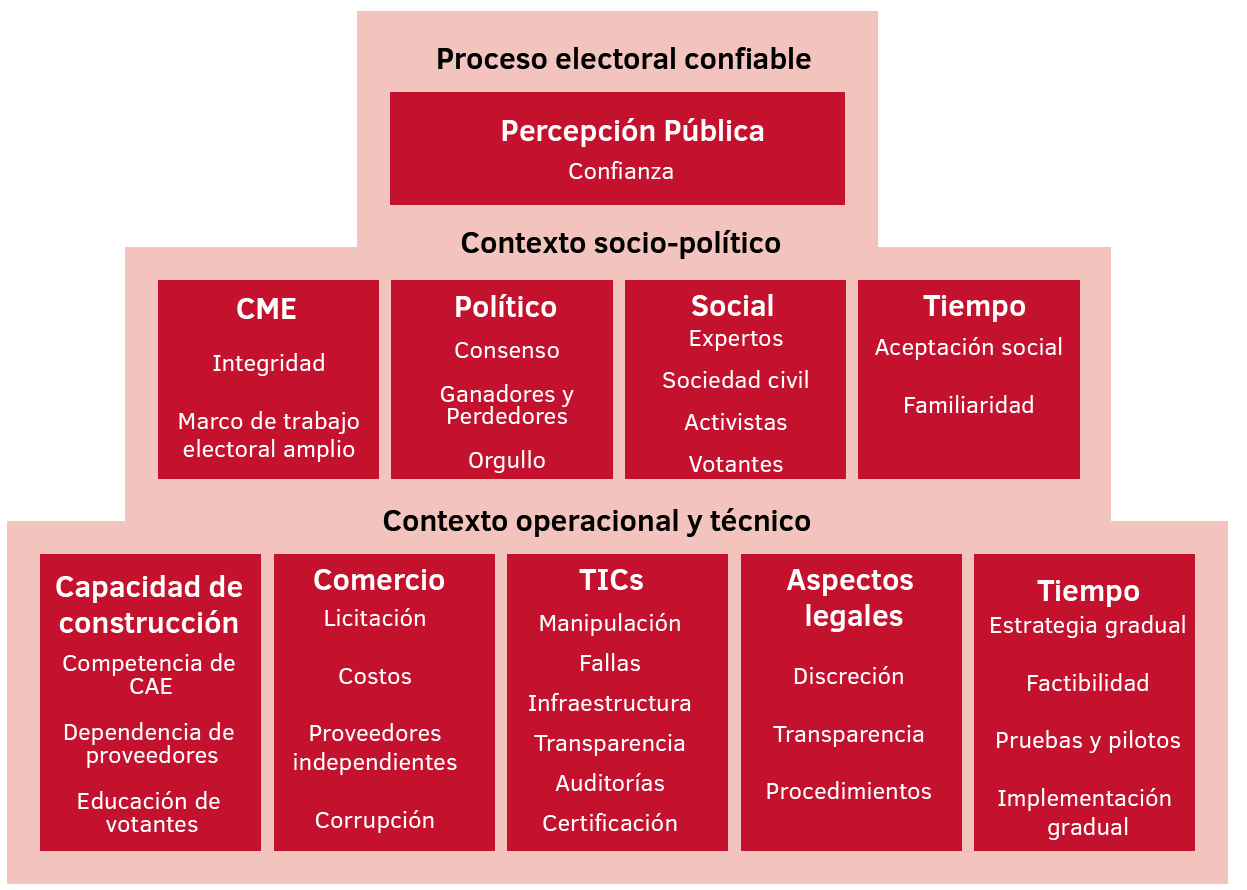
\includegraphics[width=\textwidth]{figura-piramide}
	\caption[Pirámide de confianza en el voto electrónico]{Pirámide de confianza en el voto electrónico,
	 TIC = tecnologías de información y comunicación, CAE = cuerpo de adminstración electoral, 
	adaptado de \cite{InternationalInstituteforDemocracyandElectoralAssistance2011}}
	\label{fig:piramide}
\end{figure}

Un contexto socio-politico favorable ayuda significativamente a la introducción del e-voting y 
puede temporalmente soportar problemas que pueden ocurrir en la implementación técnica. Sin embargo, debilidades
en las bases operacionales, legales o técnicas eventualmente pueden desacreditar no sólo la votación electrónica, 
sino todo el proceso eleccionario. La cancelación completa del e-voting de un país puede ser una de sus consecuencias,
como ha pasado en Alemania, Irlanda y Holanda. Un contexto socio-politico negativo crea serios riesgos, incluso cuando
las bases técnicas y operacionales están bien establecidas. Es muy difícil hacer que los sistemas de votación
electrónica sean transparentes y que sus operaciones sean entendidas en el corto y mediano plazo por una
audiencia no experta \cite{InternationalInstituteforDemocracyandElectoralAssistance2011}.

En términos técnicos, el principal desafío de la votación electrónica es
diseñar sistemas que provean un alto aseguramiento de la exactitud del resultando, mientras que
al mismo tiempo se garantice la privacidad de los votos. El problema con estos dos requerimientos es que 
están en conflicto. Tomado cada uno por separado sería sencillo de alcanzar \cite{Ryan2010}.  Incluso
resolviendo estos desafíos técnicos, la adopción en elecciones vinculantes no es sencilla, puesto que en términos 
operacionales una de las tareas más difíciles es mantener supervisión,control
y propiedad del sistema e-voting, evitando la dependencia en los proveedores. Descansar
demasiado en compañías privadas para la logística y tecnología de los sistemas no es aceptable, ya que 
se espera que el personal de administración sea capaz de intervenir de manera transparente y eficiente para
cualquier eventualidad.

Con respecto a las experiencias de adopción de la votación electrónica,  \cite{Krimmer2007} hace una revisión de más de 
100 elecciones con la opción de votación electrónica remota que muestra que si bien el e-voting ha 
llegado a niveles regionales, a niveles nacionales es un fenómeno muy raro. ``La mayoría de las otras naciones aún 
siguen en fase de experimentación. A la fecha la mayoría de los  ensayos no siguen montajes 
experimentales clásicos y están inmersos en su contexto nacional, lo cual dificulta la 
comparación y aprendizaje de otros''. Más aún, en países con adopción de votación electrónica vinculante
como Estonia y E.E.U.U, \cite{Kapczynski2009} identifica dos problemas graves en el proceso eleccionario: 

\begin{itemize}
	\item \textbf{Barrera psicológica:} El voto tradicional es visto como un gran evento, mientras que las 
		elecciones a través de Internet son vistas como algo trivial. Como se ha dicho anteriormente 
		las votaciones electrónicas requieren que todo el público tenga confianza en las herramientas y medios técnicos,
		cosa que no siempre se alcanza. En las elecciones de 2007 en Estonia, si bien la intención de 
		voto por Internet fue de mas de un 80\%, sólo poco más del 5\% de los votos emitidos provinieron de Internet.

	\item \textbf{Problemas técnicos:} En las elecciones realizadas en 2002 en E.E.U.U hubieron instancias 
		de votos perdidos e incorrectamente registrados. La escala de este fenómeno fue significante, dado que
		en algunos condados el número de aquellos votos alcanzo el 48\%.
		
\end{itemize}

Por último, en el ámbito académico existe una gran demanda para aplicar las técnicas de ingeniería apropiada
para ayudar a la correcta construcción de sistemas de e-voting confiables para poder mitigar algunas
de las consecuencias y riesgos asociados a estos. Sin embargo, no existe una clasificación detallada
de las características y limitaciones comunes de los trabajos existentes. Sin tener un estudio comprensivo,
es difícil para desarrolladores e ingenieros elegir las prácticas de desarrollo apropiadas \cite{Adida2006}. 
Considerando esto, actualmente las tendencias en la investigación se dividen en 6 líneas de trabajo, descritas
en la tabla~\ref{tab:lineas-trabajo}.

\begin{table}[h!]
\centering
\caption[Líneas de investigación de voto electrónico en la literatura]{Líneas de investigación de voto electrónico en la literatura, adaptado de  \cite{Al-Shammari2012}}
\label{tab:lineas-trabajo}
\begin{tabularx}{\textwidth}{>{\raggedright\arraybackslash}p{4cm} X} 
\toprule[1.5pt]
\bf 	Nombre							& \bf 	Descripción 	\\ \hline
	Ingeniería de requerimientos       		&	Contribuye a la definición, 
										desarrollo y estructuración de 
										requerimientos para sistemas 
										de e-voting	\\ 
	Negocios y reingeniería de procesos	&	Entender cómo implementar 
										efectivamente sistemas 
										de e-voting	\\ 
	Diseño e implementación			&	Diseño de esquemas, protocolos 
										y/o técnicas para mejorar el diseño 
										de máquinas y sistemas.	\\ 				
	Evaluación de seguridad				&	Combinar diferentes técnicas de 
										seguridad para evaluar y/o analizar 
										la situación (posture) de la 
										seguridad de los sistemas de 
										e-voting \\
	Métodos formales					&	Aplicar especificaciones formales 
										y técnicas de verificación para 
										analizar la seguridad de sistemas 
										de e-voting \\
	Métodos de verificación del voto		&	Aplicar técnicas de software o 
										hardware para asegurar que los 
										votos recolectados correspondan 
										a las elecciones de los votantes \\ 
					
\bottomrule[1.25pt]
\end {tabularx}
\end{table}

\newpage
\subsection{Protocolos de encriptación}

Los protocolos de votación electrónica suelen referirse a la manera
en que se utilizan medios criptográficos para poder llevar a cabo la elección.
Están orientados, pero no limitados, a los procesos de ejercer el voto, 
contar los votos y verificar la integridad de la elección. 

La importancia de estos protocolos de encriptación es que son críticos
para poder satisfacer los requisitos de privacidad y anonimato presentes 
en las elecciones. Dependiendo de los protocolos es posible implementar
algunos de los requisitos de las elecciones, como Verifiability o Coercion-resistance, 
pero a la vez implican restricciones que no son posibles de permitir dependiendo
del tipo de elección.

\newpage

Según \cite{NovotnyMarianInstituteofComputerScience2009}, existen 
diversas categorías de protocolos, siendo los más populares: 
\textit{blind signature schemes, homomorphic encryption schemes} y
\textit{schemes based on mixing the votes}. 
La siguiente lista los describe: \cite{Moran:2006:RUV:2165316.2165338}

\begin{itemize}

	\item \textbf {Mix-type:} Protocolos basados en mezclas. Básicamente los votantes
		encriptan sus votos con la llave pública de la autoridad eleccionaria y publica
		el texto encriptado (ciphertext) en una tabla de anuncios. Después de haber concluido
		la fase de votación, se reciben todos los textos encriptados, se desordenan y se devuelven
		en un orden aleatorio para hacer que los votos sean anónimos. Luego, se desencriptan los votos
		por la autoridad de elección para ser contados. \cite{Bernhard2013} La figura~\ref{fig:voto-cripto}
		ejemplifica este tipo de protocolos.

	\item \textbf {Blind signatures:} Una firma ciega permite al firmante ``firmar'' 
		digitalmente un documento sin saber qué es lo que se firmó. La idea 
		básica de estos protocolos es que la autoridad puede verificar públicamente
		que el voto es válido sin saber su contenido ni quién lo utilizó. 

	\item \textbf {Homomorphic:} Una función E es homomorfa si para cada x e y
		en su dominio se satisface que E(x)E(y) = E(x + y). La idea general de 
		los esquemas de voto homomorfo es que cada votante cifra su voto 
		usando una función de clave pública homomorfa, la cual es publicada 
		antes de la elección. Cada votante debe probar que su voto cifrado 
		deriva de un voto valido. Los votos son contados usando la propiedad homomorfa 
		de la función de cifrado, de modo tal que es posible contarlos sin 
		descifrarlos. Las ventajas de este método son la eficiencia y la verificabilidad: varias operaciones 
		pueden ser conducidas públicamente en los votos cifrados, por tanto 
		son verificables y pueden ser ejecutadas durante el proceso de votación
		(sin interacción de las autoridades de votación).

\end{itemize}

En la figura~\ref{fig:voto-cripto} se puede desprender cómo funcionan los protocolos basados en mezclas,
en éstos protocolos los nombres de los votantes pueden ser verificados en una base de datos con los registros
de los votantes. Luego, los encargados de la elección proceden a anonimizar los votos para luego desencriptarlos,
proveyendo de pruebas para que cualquier observador pueda verificar. Luego los resultados son publicados
para todos el público.

\begin{figure}[h!]
	\centering
	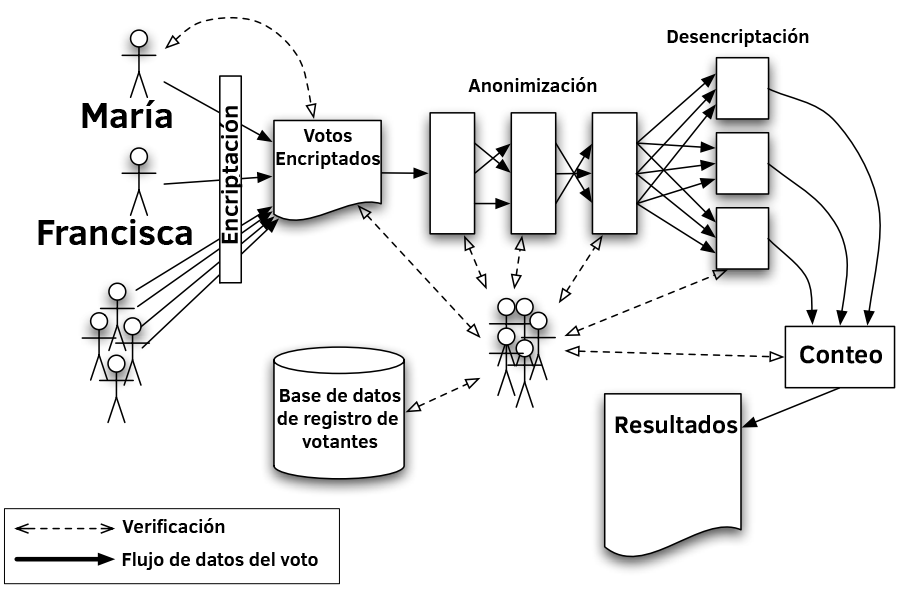
\includegraphics[width=\textwidth]{figura-voto-cripto}
	\caption[Esquema de Voto criptográfico basado en mix-net]{Esquema de Voto criptográfico basado en mix-net, adaptado de \cite{Adida2006}}
	\label{fig:voto-cripto}
\end{figure}

\section{Modelos de calidad de software}
\subsection{Definición}

La calidad de un sistema es el resultado de la calidad de los elementos
del sistema y sus interacciones. La calidad del software es el grado en el cual
el producto de software satisface necesidades implícitas y explícitas cuando son
utilizadas bajo condiciones especificadas. \cite{ISO/IEC2011}

Un modelo de calidad se entiende como ``un modelo con el objetivo
de describir, asesorar y/o predecir calidad''. Estos modelos son usados en distintas
partes del ciclo de vida del software. Durante la ingeniería de requerimientos, ellos
definen atributos de calidad y requerimientos para sistemas de software, constituyendo
un método para consensuar con el cliente qué realmente significa calidad. Durante la 
implementación, los modelos de calidad sirven como base para la modelación
y estándares de código, puesto que proveen recomendaciones directas en la 
implementación del sistema para alcanzar software de alta calidad. Por último, defectos
de calidad son encontrados durante el \textit{quality assurance} usando modelos 
de calidad \cite{Deissenboeck}.


\subsection{ISO/IEC 9126}

La ISO/IEC 9126 es un estándar dividido en 4 partes: modelo de calidad,
métricas externas, métricas internas y calidad de uso. El modelo de calidad
describe un conjunto de propiedades del software con el propósito de caracterizar
el control de calidad \cite{ISO/IEC2001}. 

El estándar identifica 6 características: \textit{Functionality}, \textit{Reliability}, \textit{Usability},
 \textit{Efficiency}, \textit{Maintainability} y \textit{Portability}. La figura~\ref{fig:caracteristicas-9126} detalla
la organización de éstas y sus subcaracterísticas.

\begin{itemize}
	\item \textbf{Functionality:} Un conjunto de atributos que se relacionan con 
	la existencia de un conjunto de funciones y sus propiedades específicas. 
	Las funciones son aquellas que satisfacen las necesidades implícitas o explícitas.
	
	\item \textbf{Reliability:} Un conjunto de atributos relacionados con la capacidad 
	del software de mantener su nivel de prestación bajo condiciones establecidas 
	durante un período establecido.
	
	\item \textbf{Usability:} Un conjunto de atributos relacionados con el esfuerzo 
	necesario para su uso, y en la valoración individual de tal uso, por un establecido 
	o implicado conjunto de usuarios.
	
	\item \textbf{Efficiency:} Conjunto de atributos relacionados con la relación entre 
	el nivel de desempeño del software y la cantidad de recursos necesitados 
	bajo condiciones establecidas.
	
	\item \textbf{Maintainability:} Conjunto de atributos relacionados con la facilidad 
	de extender, modificar o corregir errores en un sistema software.
	
	\item \textbf{Portability:} Conjunto de atributos relacionados con la capacidad 
	de un sistema software para ser transferido desde una plataforma a otra.
\end{itemize}


\begin{figure}[h!]
	\centering
	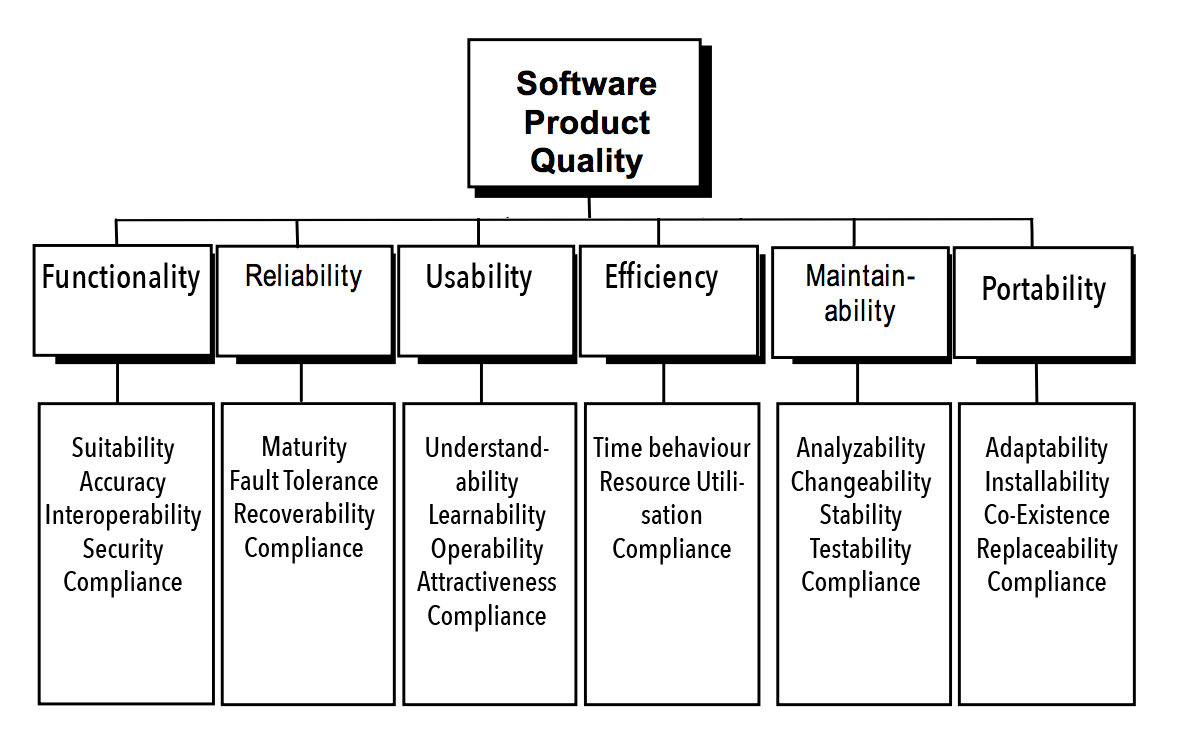
\includegraphics[width=\textwidth]{figura-9126}
	\caption[Organización de características y subcaracterísticas de estándar ISO/IEC 9126-1]{Organización de características y subcaracterísticas de estándar ISO/IEC 9126-1, adaptado de \cite{ISO/IEC2001}}
	\label{fig:caracteristicas-9126}
\end{figure}
\bigskip


\subsection{ISO/IEC 25010}

El estándar ISO/IEC 25010:2011 es una revisión del estándar
9126-1:2001. Incorpora similares características de calidad de software
con algunas modificaciones. Un modelo de calidad de producto es 
que consisten en 8 características, las cuales son subdivididas en 
subcaracterísticas, que se refieren a propiedades estáticas de software
y propiedades dinámicas de sistemas de computación.

Las características de los modelos son aplicables a cualquier tipo de software.
Las características y subcaracteristicas proveen de una terminología consistente
para la calidad de producto de software. También proveen un conjunto de característcas
de calidad las cuales pueden ser comparados con requerimientos de calidad. Los modelos
de calidad pueden ser usados para asistir la especificación y evaliacion de software 
desde distintas perspectivas relacionadas con la adquisición, requerimientos, desarrollo,
uso, evaluación, soporte, mantenimiento, aseguramiento de la calidad y auditorías de
software.

\begin{figure}[h!]	
	\centering
	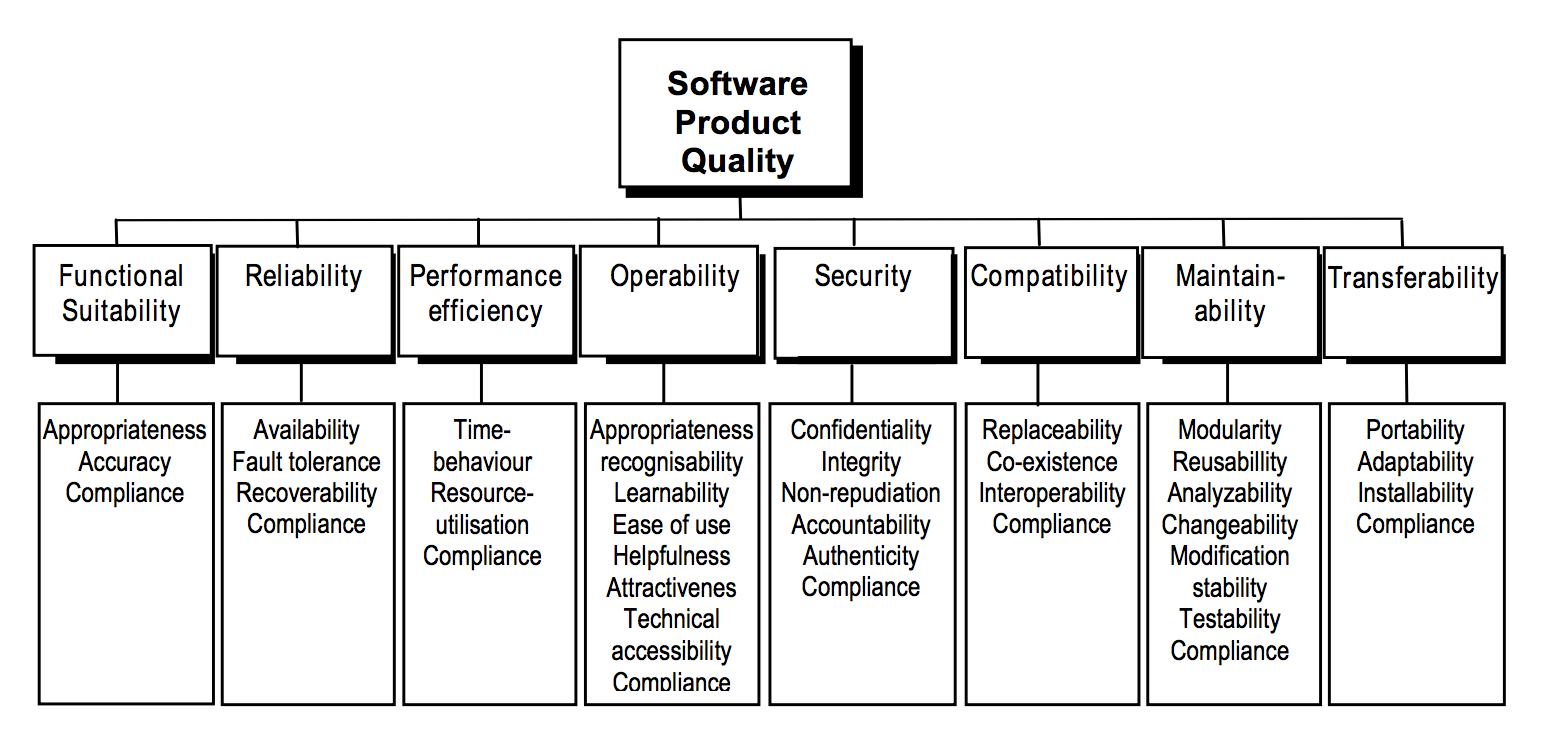
\includegraphics[width=\textwidth]{figura-25010}
	\caption[Organización de características y subcaracterísticas de calidad estándar ISO/IEC 25010]{Organización de características y subcaracterísticas de calidad estándar ISO/IEC 25010, adaptado de \cite{ISO/IEC2011}}
	\label{fig:caracteristicas-25010}
\end{figure}
\bigskip


La figura~\ref{fig:caracteristicas-25010} describe la división de características y subcaracterísticas 
del modelo de calidad. El estándar identifica 8 características: \textit{Functionality}, 
\textit{Reliability}, \textit{Operability}, \textit{Performance Efficiency}, \textit{Maintainability} y \textit{Portability}.

\begin{itemize}
	\item \textbf{Functional Suitability:} El grado en el cual el producto de software provee funciones
		que satisfacen necesidades implícitas y explícitas cuando el software es usado bajo
		condiciones específicas.
		
	\item \textbf{Reliability:} El grado en el cual el producto de software puede mantener un nivel
		específico de rendimiento cuando es usado bajo condiciones específicas.
		 	
	\item \textbf{Performance efficiency:} El grado en el cual el producto de software provee rendimiento 
		apropiado, relativo a la cantidad de recursos usados, bajo condiciones específicas.

	\item \textbf{Operability:} El grado en el cual el producto de software puede ser entendido, aprendido, usado
		y atractivo al usuario, cuando es usado bajo condiciones específicas.

	\item \textbf{Security:} La protección del sistema de acceso, uso, modificación, destrucción o revelación
		 accidental o maliciosa.

	\item \textbf{Compatibility:} La habilidad de dos o más componentes de software para intercambiar 
		información y/o para realizar sus funciones requeridas mientras usan el mismo entorno de hardware o 
		software.
		
	\item \textbf{Maintainability:} El grado en el cual el producto de software puede ser modificado. Las modificaciones
		pueden incluir correcciones, mejoras o adaptaciones al software de cambios en el entorno, y de cambios en
		sus requerimientos y especificaciones funcionales.
		
	\item \textbf{Transferability:} El grado en el cual el producto de software puede ser transferido
		de un entorno a otro.
\end{itemize}


Dada la extensión del estándar ISO/IEC 25010:2011, sólo se describirán las
subcaracterísticas que interesan a los sistemas de votación electrónica
de acuerdo a lo desprendido por distintos autores y que luego serán utlizados para
la construcción del mapeo sistemático. Esta decisión fue tomada en base a las restricciones
de este trabajo y a las recomendaciones del profesor guía. La lista a continuación con 
argumentos para justificar la elección de las 4 características: \textit{Security}, \textit{Reliability}, 
\textit{Performance efficiency} y \textit{Operability} no es exhaustiva dada la literatura revisada a lo largo de este trabajo:

\begin{itemize}
	\item \cite{Schryen2009} advierte que ``los aspectos de seguridad son considerados los más relevantes 
	en la discusión de voto electrónico en general, y en particular en el voto por internet''.
				
	\item \cite{Notations2009} define una lista exhaustiva de requerimientos de software para 
		sistemas de voto electrónico. Después de los requerimiento funcionales, hay 21 requerimientos de 
		seguridad, 8 de usabilidad, 12 de aseguramiento y 15 operacionales.
		
	\item \cite{Bryans2006} explica que para el éxito de los sistemas de voto electrónico se deben abordar ``problemas de diseño para sistemas resistentes
		a fallas, (...) complementando con mecanismos explícitos de recuperación, requerimientos de confianza en sub-sistemas y 
		preocupación por ataques de denegación de servicio, además de la necesidad de integrar las consideraciones técnicas con
		consideraciones sociales y sicológicas para determinar el perfil de amenazas, la reacción de los votantes y la efectividad de 
		los mecanismos socio-técnicos para la detección de errores y recuperación".
		
	\item \cite{Spycher2012} explica que ``(...)Esquemas que logran evitar estos ataque de coerción son llamados resistentes
		 a coerción (coecion-resistant). Para poner estos avances de segurdad en práctica, Juels et al. aún necesita hacer 
		fuertes suposiciones relativas al poder computacional de los servidores de conteo. Tales suposiciones hacen que implementar
		el esquema sea impracticable para elecciones a gran escala'.'
\end{itemize}

\begin{itemize}
	\item \textbf{Security}
		\begin{itemize}
		\item \textbf{Confidentiality:} El grado por el cual el producto de software provee protección
			para accesos no autorizados de datos o información, sean accidentales o deliberados.
		\item \textbf{Integrity:} El grado por el cual la exactitud e integridad de los activos (assets) están protegidos.
		\item \textbf{Non-repudiation:} El grado por el cual las acciones o eventos pueden ser probados de haber sido 
			cometidos, de forma tal que los eventos o acciones no pueden ser descartados (repudiated) después.		
		\item \textbf{Accountability:} El grado por el cual las acciones de una entidad pueden ser rastreadas
			únicamente a la entidad. 
		\item \textbf{Authenticity:} El grado por el cual la identidad de un sujeto o recurso puede ser probado 
			de ser quién dice ser.
		\item \textbf{Security Compliance:} El grado por el cual el producto de software adhiere a estándares,
			convenciones o regulaciones relativas a la seguridad.
		\end{itemize}
		
	\item \textbf{Reliability}
		\begin{itemize}
		\item \textbf{Availability:} El grado por el cual un component de software es operacional y disponible
			cuando es requerido su uso.
		\item \textbf{Fault tolerance:} El grado por el cual el producto de software puede mantener un nivel
			especificado de rendimiento en caso de fallos de software o la violación de sus interfaces especificadas.
		\item \textbf{Reliability compliance:} El grado por el cual el producto de software adhiere a estándares, convenciones
			o regulaciones relativas a la confiabilidad.
		\end{itemize}
	
	\item \textbf{Performance efficiency}
		\begin{itemize}
		\item \textbf{Time behaviour:} El grado por el cual el producto de software provee tasas de rendimiento, tiempos de respuesta
			y proceso apropiados cuando realiza sus funciones, bajo condiciones específicas.
		\item \textbf{Resource utilisation:} El grado por el cual el producto de software usa cantidades y tipos
			apropiados de recursos cuando el software realiza sus funciones bajo condiciones específicas.
		\item \textbf{Performance compliance:} El grado por el cual el producto de software adhiere a estándares, convenciones
			o regulaciones relativas a la eficiencia de rendimiento.
		\end{itemize}
		
	\item \textbf{Operability}
		\begin{itemize}
		\item \textbf{Ease of Use:} El grado por el cual el producto de software hace fácil a sus usuarios
			operarlo y controlarlo.
		\item \textbf{Appropriateness recognisability:} El grado por el cual el producto de software habilita a sus
			usuarios a reconocer si el software es apropiado para sus necesidades.
		\item \textbf{Learnability:} El grado por el cual el producto de software habilita a los usuarios a aprender
			sobre la aplicación.
		\item \textbf{Helpfulness:} El grado por el cual el producto de software provee ayuda cuando los
			usuarios necesitan asistencia.
		\item \textbf{Attractiveness:}  El grado por el cual el producto de software es atractivo para el usuario.
		\item \textbf{Technical accessibility:}  El grado de operabilidad del software por usuarios con
			discapacidades específicas.
		\item \textbf{Operability compliance:} El grado por el cual el producto de software adhiere a estándares, convenciones
			o regulaciones relativas a la operabilidad.
		\end{itemize}

		
\end{itemize}


\cleardoublepage
\section{Ingeniería de requerimientos}
\subsection{Definición e importancia}

La ingeniería de requerimientos se refiere al proceso de formular, documentar
y mantener requerimientos de software \cite{Sommerville1998}. El SWEBOK V3
se refiere a la ingeniería de requerimientos como el proceso que aborda la elicitación, 
análisis,especificación y validación de requerimientos de software como también
la gestión de requerimientos durante todo el ciclo de vida del software \cite{IEEEComputerSociety2013}.

Básicamente, un requerimiento de software es una propiedad que 
debe ser exhibida por el software en algún nivel para poder resolver un problema. Los 
requerimientos son clasificados principalmente en dos tipos: funcionales y no funcionales.


\subsection{Requerimientos funcionales}

Los requerimientos funcionales describen las funciones que el software ejecuta. 
Algunas veces son conocidas como capacidades o características.

Requerimientos funcionales describen las funciones que el software ejecutará. Algunas 
veces son nombradas como capacidades o características. Un requerimiento funcional
también puede ser descrito como el cual un conjunto finito de pasos de prueba puede
ser escrito para validar su comportamiento \cite{IEEEComputerSociety2013}.

\subsection{Requerimientos no-funcionales}

La definición del término de requerimientos no funcionales
no está clara. En la literatura encontramos distintas definiciones
(tabla~\ref{tab:definiciones-nfr}). Existe un consenso en que todas 
las definiciones de requerimientos no funcionales se basan en 
los términos \textit{propiedad o característica},
\textit{atributo},\textit{calidad},\textit{restriccion} y \textit{rendimiento} 
aún cuando no existe un consenso en cuánto a los conceptos 
que éstos términos denotan \cite{Glinz2007}.

Según las definiciones más actuales y generales, los requerimientos no funcionales
son aquellas que actúan para restringir la solución. Requerimientos no funcionales
algunas veces son llamadas restrincciones o requerimientos de calidad. Pueden ser
clasificadas de acuerdo a las características de modelos de calidad, como requerimientos
de rendimiento, confiabilidad, interoperabilidad, seguridad, mantenibilidad, etc. \cite{IEEEComputerSociety2013}

\begin{table}
\centering
\renewcommand{\arraystretch}{1}
\caption{Distintas definiciones de requerimientos no funcionales}
\label{tab:definiciones-nfr}
\begin{tabularx}{\textwidth}{p{2.5cm} X} 
\toprule[1.5pt]
	\bf 	Fuente				& 	\bf 	Definición  	\\
	\cite{I.JacobsonG.Booch}	& 	A requirement that specifies system properties, such as 
								environmental and implementation constraints, performance, 
								platform dependencies, maintainability, extensibility, and reliability. 
								A requirement that specifies physical constraints on a functional requirement \\ 								
	\cite{Sommerville1998}		&	Requirements which are not specifically concerned with the functionality of a system. 
								They place restrictions on the product being developed and the 
								development process, and they specify external constraints 
								that the product must meet. \\	
	\cite{Mylopoulos1992}		&	“... global requirements on its development or operational cost, performance, 
								reliability, maintainability, portability, robustness, and the like. (...) 
								There is not a formal definition or a complete list of nonfunctional requirements.” \\
\bottomrule[0.5pt]
\end{tabularx}
\centerline{Adaptado de \cite{Glinz2007}}
\end{table}
\bigskip

En este trabajo consideramos que las características y subcaracterísticas planteadas en 
el ISO/IEC 25010 están relacionadas con requerimientos no funcionales ya que se basan
en atributos de calidad que los sistemas de votación electrónica pueden satisfacer.


\newpage
\section{Mapeo sistemático}

\subsection{Concepto}

El mapeo sistemático \cite{Budgen2007} es un método robusto y repetible usado particularmente para
responder metódicamente de forma objetiva y libre de sesgo preguntas de investigación,
identificando los principales estudios que pueden contener información relevante (búsqueda), 
seleccionando los estudios pertinentes después de mayor revisión (inclusión/exclusión) y
donde es apropiado, realizar una evaluación de calidad de los estudios seleccionado (sesgo/validez).

\subsection{Definición de protocolo aplicado a IS}

En el dominio de la ingeniería de software, \cite{Petersen2007} ha propuesto un protocolo
a seguir para la conducción de mapeos sistemáticos. En la figura~\ref{fig:pasos-ms} se muestra un esquema
general.

\begin{figure}[h!]
	\centering
	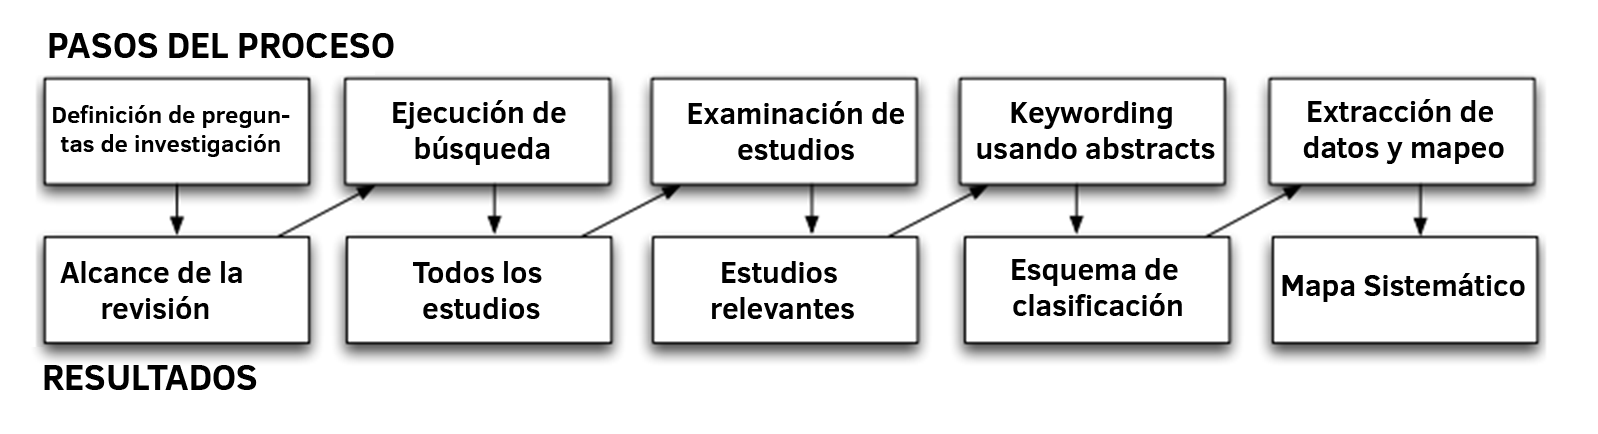
\includegraphics[width=\textwidth]{petersen-mappingsteps}
	\caption[Pasos del proceso de mapeo sistemático]{Pasos del proceso de mapeo sistemático, adaptado de \cite{Petersen2007}}
	\label{fig:pasos-ms}
\end{figure}


\begin{description}
\item[Definición de las preguntas de investigación:] Al ser el objetivo de un mapeo sistemático
	obtener un resumen de un tópico, se deben establecer  preguntas de investigación que 
	se alineen con este objetivo y al mismo tiempo puedan ser respondidas en términos 
	cuantitativos. 

\item[Ejecución de búsqueda:] Los estudios a analizar son identificados mediante la 
consulta de bases de datos científicas, usando cadenas de búsquedas estructuradas
en base a los conceptos clave del tópico y las preguntas de investigación.

\item[Examinación de estudios:] Utilizando los criterios de inclusión y exclusión 
podemos descartar estudios que mencionen nuestro tema principal de forma 
tangencial o que esten ajenos a éste.

\item[Palabras clave de abstracts:] Se clasifican los estudios de acuerdo a sus abstracts
asignándoles palabras clave, de forma tal de acelerar la extracción de datos 

\item[Extracción de datos y mapeo:] Dados los estudios pertinentes y las clasificaciones
mediante palabras claves, es en esta etapa en donde se extraen datos y a la vez se 
modifica el esquema de clasificaciones, luego se enfoca en obtener las frecuencias
para publicarlas en la tabla final.

\end{description}

